\documentclass[a4paper,12pt,landscape,twocolumn]{article}

\usepackage{préambule}
\usepackage{clipboard}

\setmathfont[range=it]{Tex Gyre Schola Math}

\geometry{left=1cm}
\setlength{\columnsep}{0.8cm}

\newcommand{\drawhouseat}[1]{
	\draw[draw=brown,line width=0.5mm] (#1) node[mynode] {} -- ++(0.5,-0.866) node[mynode] {} -- ++(0,-1) node[mynode] {} -- ++(-1,0) node[mynode] {} -- ++(0,1) node[mynode] {} -- cycle;
}

\TitreDActivite{Activité : La suite de maisons}

\begin{document}

\Copy{Contenu}{
	\maketitle

	On réalise des maisons avec des cure-dents :

	\begin{center}
		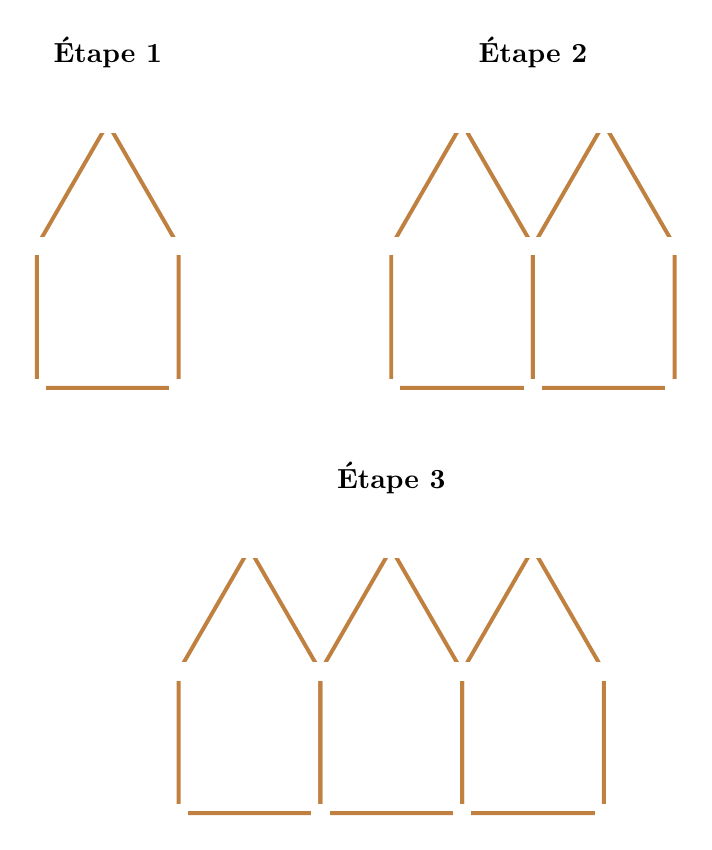
\begin{tikzpicture}[
				scale=1.8,
				mynode/.style={rectangle,fill=white,anchor=center}]
			\node at (0, 0) {\textbf{Étape 1}};
			\drawhouseat{0,-0.5}

			\node at (3, 0) {\textbf{Étape 2}};
			\drawhouseat{2.5,-0.5}
			\drawhouseat{3.5,-0.5}

			\node at (2, -3) {\textbf{Étape 3}};
			\drawhouseat{1,-3.5}
			\drawhouseat{2,-3.5}
			\drawhouseat{3,-3.5}
		\end{tikzpicture}
	\end{center}

	\begin{enumerate}
		\item Combien de cure-dents faut-il pour les étapes 1, 2 et 3 ?
		\item Combien de cure-dents faut-il pour réaliser 25 maisons ?
		\item Combien de cure-dents faut-il pour réaliser 2015 maisons ?
		\item Henri affirme qu'avec 109 cure-dents, il construira des maisons et qu'il ne restera aucun cure-dent. A-t-il raison ?
	\end{enumerate}
}

\newpage

\Paste{Contenu}

\end{document}